\documentclass[11pt]{article}
\usepackage[paper=letterpaper,margin=1in]{geometry}

\usepackage[parfill]{parskip}
\usepackage{amsmath}
\usepackage{graphicx}
\usepackage{tikz}
\usepackage[
backend=biber,
citestyle=alphabetic,
style=alphabetic,
sorting=ynt
]{biblatex}
\addbibresource{sample.bib}

\begin{document}
\thispagestyle{empty}
\title{CS 310 \\
\large Assignment 321}
\date{March 23, 2017}
\author{Cameron Moberg}
\maketitle

There are several ways to solve the closest-pair problem; the two done in this analysis are the brute force method and the divide and conquer method. The purpose of this study is to perform an empirical analysis of the two methods.

For both methods, the value for $n$ is taken to be the number of points in the plane.

\section{Brute Force}
To analyze the brute force algorithm, we chose calculating the distance on line 67 as the basic operation because this happens most frequently, is the most expensive, and is the philosophical heart of this algorithm.

An empirical analysis of running the algorithm for multiple values of
$n$ produces the results shown below. Standard function $f(n) = n^2$ with constant multipliers, has been added to
illustrate the analysis.

\begin{center}
    % GNUPLOT: LaTeX picture with Postscript
\begingroup
  \makeatletter
  \providecommand\color[2][]{%
    \GenericError{(gnuplot) \space\space\space\@spaces}{%
      Package color not loaded in conjunction with
      terminal option `colourtext'%
    }{See the gnuplot documentation for explanation.%
    }{Either use 'blacktext' in gnuplot or load the package
      color.sty in LaTeX.}%
    \renewcommand\color[2][]{}%
  }%
  \providecommand\includegraphics[2][]{%
    \GenericError{(gnuplot) \space\space\space\@spaces}{%
      Package graphicx or graphics not loaded%
    }{See the gnuplot documentation for explanation.%
    }{The gnuplot epslatex terminal needs graphicx.sty or graphics.sty.}%
    \renewcommand\includegraphics[2][]{}%
  }%
  \providecommand\rotatebox[2]{#2}%
  \@ifundefined{ifGPcolor}{%
    \newif\ifGPcolor
    \GPcolorfalse
  }{}%
  \@ifundefined{ifGPblacktext}{%
    \newif\ifGPblacktext
    \GPblacktexttrue
  }{}%
  % define a \g@addto@macro without @ in the name:
  \let\gplgaddtomacro\g@addto@macro
  % define empty templates for all commands taking text:
  \gdef\gplbacktext{}%
  \gdef\gplfronttext{}%
  \makeatother
  \ifGPblacktext
    % no textcolor at all
    \def\colorrgb#1{}%
    \def\colorgray#1{}%
  \else
    % gray or color?
    \ifGPcolor
      \def\colorrgb#1{\color[rgb]{#1}}%
      \def\colorgray#1{\color[gray]{#1}}%
      \expandafter\def\csname LTw\endcsname{\color{white}}%
      \expandafter\def\csname LTb\endcsname{\color{black}}%
      \expandafter\def\csname LTa\endcsname{\color{black}}%
      \expandafter\def\csname LT0\endcsname{\color[rgb]{1,0,0}}%
      \expandafter\def\csname LT1\endcsname{\color[rgb]{0,1,0}}%
      \expandafter\def\csname LT2\endcsname{\color[rgb]{0,0,1}}%
      \expandafter\def\csname LT3\endcsname{\color[rgb]{1,0,1}}%
      \expandafter\def\csname LT4\endcsname{\color[rgb]{0,1,1}}%
      \expandafter\def\csname LT5\endcsname{\color[rgb]{1,1,0}}%
      \expandafter\def\csname LT6\endcsname{\color[rgb]{0,0,0}}%
      \expandafter\def\csname LT7\endcsname{\color[rgb]{1,0.3,0}}%
      \expandafter\def\csname LT8\endcsname{\color[rgb]{0.5,0.5,0.5}}%
    \else
      % gray
      \def\colorrgb#1{\color{black}}%
      \def\colorgray#1{\color[gray]{#1}}%
      \expandafter\def\csname LTw\endcsname{\color{white}}%
      \expandafter\def\csname LTb\endcsname{\color{black}}%
      \expandafter\def\csname LTa\endcsname{\color{black}}%
      \expandafter\def\csname LT0\endcsname{\color{black}}%
      \expandafter\def\csname LT1\endcsname{\color{black}}%
      \expandafter\def\csname LT2\endcsname{\color{black}}%
      \expandafter\def\csname LT3\endcsname{\color{black}}%
      \expandafter\def\csname LT4\endcsname{\color{black}}%
      \expandafter\def\csname LT5\endcsname{\color{black}}%
      \expandafter\def\csname LT6\endcsname{\color{black}}%
      \expandafter\def\csname LT7\endcsname{\color{black}}%
      \expandafter\def\csname LT8\endcsname{\color{black}}%
    \fi
  \fi
    \setlength{\unitlength}{0.0500bp}%
    \ifx\gptboxheight\undefined%
      \newlength{\gptboxheight}%
      \newlength{\gptboxwidth}%
      \newsavebox{\gptboxtext}%
    \fi%
    \setlength{\fboxrule}{0.5pt}%
    \setlength{\fboxsep}{1pt}%
\begin{picture}(7200.00,5040.00)%
    \gplgaddtomacro\gplbacktext{%
      \csname LTb\endcsname%
      \put(1342,704){\makebox(0,0)[r]{\strut{}$0$}}%
      \put(1342,1163){\makebox(0,0)[r]{\strut{}$500000$}}%
      \put(1342,1623){\makebox(0,0)[r]{\strut{}$1\times10^{6}$}}%
      \put(1342,2082){\makebox(0,0)[r]{\strut{}$1.5\times10^{6}$}}%
      \put(1342,2542){\makebox(0,0)[r]{\strut{}$2\times10^{6}$}}%
      \put(1342,3001){\makebox(0,0)[r]{\strut{}$2.5\times10^{6}$}}%
      \put(1342,3460){\makebox(0,0)[r]{\strut{}$3\times10^{6}$}}%
      \put(1342,3920){\makebox(0,0)[r]{\strut{}$3.5\times10^{6}$}}%
      \put(1342,4379){\makebox(0,0)[r]{\strut{}$4\times10^{6}$}}%
      \put(1474,484){\makebox(0,0){\strut{}$0$}}%
      \put(2007,484){\makebox(0,0){\strut{}$200$}}%
      \put(2540,484){\makebox(0,0){\strut{}$400$}}%
      \put(3073,484){\makebox(0,0){\strut{}$600$}}%
      \put(3606,484){\makebox(0,0){\strut{}$800$}}%
      \put(4139,484){\makebox(0,0){\strut{}$1000$}}%
      \put(4671,484){\makebox(0,0){\strut{}$1200$}}%
      \put(5204,484){\makebox(0,0){\strut{}$1400$}}%
      \put(5737,484){\makebox(0,0){\strut{}$1600$}}%
      \put(6270,484){\makebox(0,0){\strut{}$1800$}}%
      \put(6803,484){\makebox(0,0){\strut{}$2000$}}%
      \put(4139,850){\rotatebox{12}{\makebox(0,0)[l]{\strut{}$1/3n^2$}}}%
      \put(3500,1350){\rotatebox{32}{\makebox(0,0)[l]{\strut{}$n^2$}}}%
    }%
    \gplgaddtomacro\gplfronttext{%
      \csname LTb\endcsname%
      \put(176,2541){\rotatebox{-270}{\makebox(0,0){\strut{}Operation Count}}}%
      \put(4138,154){\makebox(0,0){\strut{}Input Size}}%
      \put(4138,4709){\makebox(0,0){\strut{}Empirical Analysis of Brute Force Closest Pair Problem}}%
    }%
    \gplbacktext
    \put(0,0){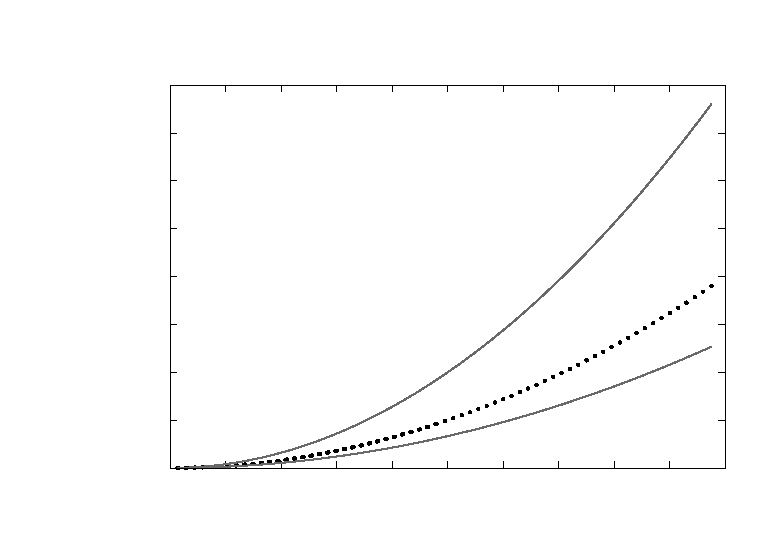
\includegraphics{output_bf}}%
    \gplfronttext
  \end{picture}%
\endgroup

\end{center}

An examination of the code itself explains the empirical results when we observe that there is a doubly-nested for-loop that iterates over the input size. Therefore, since the brute force algorithm is deterministic we conclude that the algorithm is described by

\[
T(n) \in \Theta( n^{2} )
\]

This analysis agrees with our author, however, in this case the elementary operation is calculating the squared distance, rather than the square root, which is only calculated once instead of every iteration. This only speeds up the algorithm by a constant factor, not impacting the efficiency class \cite{levit}.

\section{Divide and Conquer}
To analyze the divide and conquer algorithm, we chose the sort method on lines 122--124 as the basic operation since it is by far the most expensive operation compared to all other possible choices. After research into the \texttt{std::sort} function that C++11 uses it has been determined that the sorting algorithm used is of the runtime complexity $O(n\log n)$\cite{cplus}. Since we cannot (easily) edit the \texttt{std::sort} function, we must assume that the basic operations after each sort is increased by an $n\log n$ amount of operations, where $n$ is the number of elements sorted.

There is also the chance that all the points are included in the strip between the left and right sets of points. This makes it seem like we must use the brute force method on them which would make the local work $n^2$. However, due to the geometry of the closest-pair problem, we only need to check the 6 closest pairs. This is because of the constraint that for any point, $p$, we are only interested in the other points that are at most $\delta$ distance away, where $\delta$ is the calculated distance from earlier calculations. Shown below is a geometric example of this concept.
\begin{center}
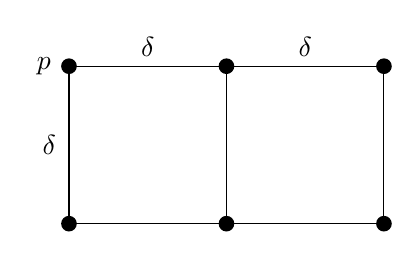
\begin{tikzpicture}
\draw (0,0) -- (4,0) -- (4,2) -- (0,2) -- (0,0);
\draw (2,2) -- (2,0);
\node at (1,2.25) {$\delta$};
\node at (3,2.25) {$\delta$};
\node at (-.25,1) {$\delta$};
\node[circle, fill, inner sep=2pt, label=left:$p$] at(0,2){};
\node[circle, fill, inner sep=2pt] at(2,2){};
\node[circle, fill, inner sep=2pt] at(2,0){};
\node[circle, fill, inner sep=2pt] at(0,0){};
\node[circle, fill, inner sep=2pt] at(4,2){};
\node[circle, fill, inner sep=2pt] at(4,0){};
\end{tikzpicture}
\end{center}
Notice how at most there are 5 other points in the $2\delta$ by $\delta$ rectangle. Showing we only need to check at most the next 6 pairs, meaning at most $6n$ comparisons are needed to check all pairs in the strip \cite{levit}.

\clearpage
An empirical analysis of running the algorithm for multiple values of
$n$ produces the results shown below. The standard function $f(n) = n\log^2 n$ with constant multipliers, has been added to
illustrate the analysis.

\begin{center}
    % GNUPLOT: LaTeX picture with Postscript
\begingroup
  \makeatletter
  \providecommand\color[2][]{%
    \GenericError{(gnuplot) \space\space\space\@spaces}{%
      Package color not loaded in conjunction with
      terminal option `colourtext'%
    }{See the gnuplot documentation for explanation.%
    }{Either use 'blacktext' in gnuplot or load the package
      color.sty in LaTeX.}%
    \renewcommand\color[2][]{}%
  }%
  \providecommand\includegraphics[2][]{%
    \GenericError{(gnuplot) \space\space\space\@spaces}{%
      Package graphicx or graphics not loaded%
    }{See the gnuplot documentation for explanation.%
    }{The gnuplot epslatex terminal needs graphicx.sty or graphics.sty.}%
    \renewcommand\includegraphics[2][]{}%
  }%
  \providecommand\rotatebox[2]{#2}%
  \@ifundefined{ifGPcolor}{%
    \newif\ifGPcolor
    \GPcolorfalse
  }{}%
  \@ifundefined{ifGPblacktext}{%
    \newif\ifGPblacktext
    \GPblacktexttrue
  }{}%
  % define a \g@addto@macro without @ in the name:
  \let\gplgaddtomacro\g@addto@macro
  % define empty templates for all commands taking text:
  \gdef\gplbacktext{}%
  \gdef\gplfronttext{}%
  \makeatother
  \ifGPblacktext
    % no textcolor at all
    \def\colorrgb#1{}%
    \def\colorgray#1{}%
  \else
    % gray or color?
    \ifGPcolor
      \def\colorrgb#1{\color[rgb]{#1}}%
      \def\colorgray#1{\color[gray]{#1}}%
      \expandafter\def\csname LTw\endcsname{\color{white}}%
      \expandafter\def\csname LTb\endcsname{\color{black}}%
      \expandafter\def\csname LTa\endcsname{\color{black}}%
      \expandafter\def\csname LT0\endcsname{\color[rgb]{1,0,0}}%
      \expandafter\def\csname LT1\endcsname{\color[rgb]{0,1,0}}%
      \expandafter\def\csname LT2\endcsname{\color[rgb]{0,0,1}}%
      \expandafter\def\csname LT3\endcsname{\color[rgb]{1,0,1}}%
      \expandafter\def\csname LT4\endcsname{\color[rgb]{0,1,1}}%
      \expandafter\def\csname LT5\endcsname{\color[rgb]{1,1,0}}%
      \expandafter\def\csname LT6\endcsname{\color[rgb]{0,0,0}}%
      \expandafter\def\csname LT7\endcsname{\color[rgb]{1,0.3,0}}%
      \expandafter\def\csname LT8\endcsname{\color[rgb]{0.5,0.5,0.5}}%
    \else
      % gray
      \def\colorrgb#1{\color{black}}%
      \def\colorgray#1{\color[gray]{#1}}%
      \expandafter\def\csname LTw\endcsname{\color{white}}%
      \expandafter\def\csname LTb\endcsname{\color{black}}%
      \expandafter\def\csname LTa\endcsname{\color{black}}%
      \expandafter\def\csname LT0\endcsname{\color{black}}%
      \expandafter\def\csname LT1\endcsname{\color{black}}%
      \expandafter\def\csname LT2\endcsname{\color{black}}%
      \expandafter\def\csname LT3\endcsname{\color{black}}%
      \expandafter\def\csname LT4\endcsname{\color{black}}%
      \expandafter\def\csname LT5\endcsname{\color{black}}%
      \expandafter\def\csname LT6\endcsname{\color{black}}%
      \expandafter\def\csname LT7\endcsname{\color{black}}%
      \expandafter\def\csname LT8\endcsname{\color{black}}%
    \fi
  \fi
    \setlength{\unitlength}{0.0500bp}%
    \ifx\gptboxheight\undefined%
      \newlength{\gptboxheight}%
      \newlength{\gptboxwidth}%
      \newsavebox{\gptboxtext}%
    \fi%
    \setlength{\fboxrule}{0.5pt}%
    \setlength{\fboxsep}{1pt}%
\begin{picture}(7200.00,5040.00)%
    \gplgaddtomacro\gplbacktext{%
      \csname LTb\endcsname%
      \put(946,704){\makebox(0,0)[r]{\strut{}$0$}}%
      \put(946,1112){\makebox(0,0)[r]{\strut{}$500$}}%
      \put(946,1521){\makebox(0,0)[r]{\strut{}$1000$}}%
      \put(946,1929){\makebox(0,0)[r]{\strut{}$1500$}}%
      \put(946,2337){\makebox(0,0)[r]{\strut{}$2000$}}%
      \put(946,2746){\makebox(0,0)[r]{\strut{}$2500$}}%
      \put(946,3154){\makebox(0,0)[r]{\strut{}$3000$}}%
      \put(946,3562){\makebox(0,0)[r]{\strut{}$3500$}}%
      \put(946,3971){\makebox(0,0)[r]{\strut{}$4000$}}%
      \put(946,4379){\makebox(0,0)[r]{\strut{}$4500$}}%
      \put(1078,484){\makebox(0,0){\strut{}$0$}}%
      \put(1651,484){\makebox(0,0){\strut{}$200$}}%
      \put(2223,484){\makebox(0,0){\strut{}$400$}}%
      \put(2796,484){\makebox(0,0){\strut{}$600$}}%
      \put(3368,484){\makebox(0,0){\strut{}$800$}}%
      \put(3941,484){\makebox(0,0){\strut{}$1000$}}%
      \put(4513,484){\makebox(0,0){\strut{}$1200$}}%
      \put(5086,484){\makebox(0,0){\strut{}$1400$}}%
      \put(5658,484){\makebox(0,0){\strut{}$1600$}}%
      \put(6231,484){\makebox(0,0){\strut{}$1800$}}%
      \put(6803,484){\makebox(0,0){\strut{}$2000$}}%
      \put(2796,1766){\rotatebox{37}{\makebox(0,0)[l]{\strut{}1/3 nlog(n)}}}%
      \put(2796,875){\rotatebox{12}{\makebox(0,0)[l]{\strut{}1/10 nlog(n)}}}%
    }%
    \gplgaddtomacro\gplfronttext{%
      \csname LTb\endcsname%
      \put(176,2541){\rotatebox{-270}{\makebox(0,0){\strut{}Operation Count}}}%
      \put(3940,154){\makebox(0,0){\strut{}Input Size}}%
      \put(3940,4709){\makebox(0,0){\strut{}Empirical Analysis of Brute Force Closest Pair Problem}}%
    }%
    \gplbacktext
    \put(0,0){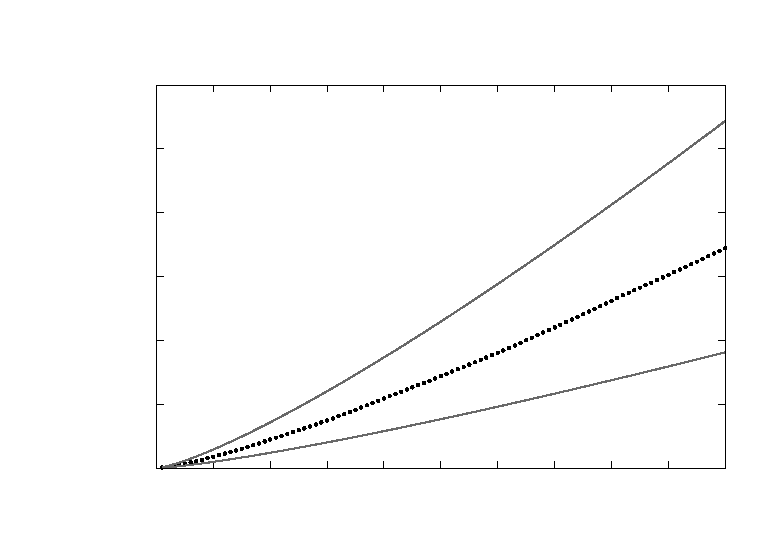
\includegraphics{output_dc}}%
    \gplfronttext
  \end{picture}%
\endgroup

\end{center}

An examination of the code itself explains the empirical results when we observe that this algorithm is recursive, lending us the ability to use the Master Theorem, which is of the form
\[
	T(n)=aT(\frac{n}{b}) + f(n) \text{ where } a \geq 1, b > 1, \text{ and } d \geq 0
\]
	
The divide and conquer algorithm has two recursive calls where each recursive call operates on half of the input. As previously stated, the local work ($f(n)$) for this algorithm is \texttt{std::sort}, which is $( n\log n )$. Additionally, there is no official documentation stating the best case runtime of C++11's sorting algorithm, so our analysis must use Big-$O$ instead of Big-$\Theta$. Since $f(n)\in O(n\log n)$ we cannot use the Master Theorem traditionally, and must use a special case where \\ \\
	if it is true for some constant, $k\geq 0$, such that:

\[	f(n) = \Theta(n^c\log^kn) \text{ where } c=\log_ba
\]
	then:
\[	
T(n) = \Theta(n^c\log^{k+1}n)
\]

 Thus, after applying this case of the Master Theorem with $c=\log_22=1$ and $k=1$ (since $f(n)=n\log n=n^{\log_22}\log^1n$) we arrive at $T(n)=O(n\log^2n$) \cite{algo}.
Seeing that the divide and conquer algorithm always runs to completion and the best-case scenario is not offered we conclude, from the  Master Theorem, that the algorithm is described by
\[
T(n) \in O( n \log^2n)
\]
We can infer, however, the possibilities of what the Big-$\Omega$ for \texttt{std::sort} could be. The efficiency of this algorithm is determined by the local work: \texttt{std::sort} ($f(n)$ from now on). By observation, we see that $f(n)\in \Omega(n\log n$), or $f(n) \in \Omega(n)$. Notice that $f(n) \notin \Omega(1)$  because sorting algorithms must process the entire input to ensure it is sorted. Also notice that $f(n)$ cannot be of a worse complexity than $\Omega(n\log n)$ because it has already been determined that $f(n)\in O(n\log n)$. So from the two possible scenarios shown above there are two possible Big-$\Omega$ runtimes for $T(n)$. Consider the following cases.

\textbf{Case 1:} $f(n) \in \Omega(n)$\\
 In this case we can use the Master's Theorem traditionally with $a=2,b=2,d=1$ showing the entire divide and conquer algorithm would be of the form
\[
T(n) \in O( n \log^2n)
\]
\[
T(n) \in \Omega(n \log n)
\]
\textbf{Case 2:} $f(n) \in \Omega(n\log n$)\\
 In this case both the Big-$O$ and Big-$\Omega$ will be the same efficiency, tightening the bound to Big-$\Theta$. After using the special case of the Master Theorem, it can be shown that algorithm would be of the form
\begin{center}
$T(n) \in \Theta(n\log^2n$)
\end{center}
\vspace{10 mm}

Unfortunately, neither scenario agrees with our author's analysis who determined the algorithm was
\begin{center}
$T(n) \in \Theta( n\log n$)
\end{center}
This is because the author states that, ``The algorithm spends linear time both for dividing the problem into two problems half the size and combining the obtained solutions"\cite{levit}. However, the author does not account for the fact that the points must be sorted by $Y$ coordinate every recursive call. As stated above sorting is $O(n\log n)$ which will dominate the linear work. Since the local work has changed, the author's calculated $f(n)=n$ should now be $f(n)=n\log n$, which changes the runtime efficiency of this algorithm.
\nocite{*}
\clearpage
\printbibliography
\end{document}